\chapter{Introduction}
The TypeDLT is a new TRNSYS component dedicated to daylighting analysis of Complex Fenestration Systems (CFS).  The tool is able to perform dynamic daylighting simulations using the Bidirectional Scattering Distribution Function (BSDF) that characterize the CFS.   
TypeDLT implements RADIANCE, a validated software for daylighting simulation, within TRNSYS, that in its standard configuration and use provides thermal simulations. In particular, the calculation algorithm implemented is the Three-Phase Method (3PM). This method allows to perform fast simulation climate-based using the BSDF data in input. 
The code, which defines the TypeDLT, contains only the functions needed to launch the 3PM. The control algorithm is maintained outside the TypeDLT in order to let the user a great flexibility in the control strategy definition. 

\section{TRNSYS}
TRNSYS \cite{trnsys} is a complete and extensible simulation environment for the transient simulation of systems, including multi-zone buildings. One of the key factors in TRNSYS is its modular architecture based on DLL (Dynamic-link library) concept. Thanks to this feature, user and third-party developers may easily add custom component models using common programming language (e.g. C, C\texttt{++}, FORTRAN, etc.).

\section{Radiance} 

Radiance \cite{radiance} is a software developed at the Environmental Energy Technologies Division of Lawrence Berkeley National Laboratory in Berkeley, California, by Greg Ward and the Lighting Systems Research group. It is an accurate tool for predict the visible radiation in a space using climate-based approach even on an annual basis. Radiance uses the back ray tracing approach that consist in following the light path (specular reflected, transmitted and refracted) from the reception point (eyes or sensors) into the scene to the light source.\\
In the practice is consider the best and more flexible software for lighting simulation, in fact is used as calculation engine in the most lighting design software available. It is also the most validate lighting simulation tool.

\subsection{Three-Phase Method} \label{sec:3ph}

The Three-Phase Method \cite{3ph1,3ph2} is an algorithm developed in Radiance that perform hourly/annually daylighting simulation for complex fenestration system and light pipes. The name is due to the sub-division of light path in three step (figure \ref{img1:3pm}) defined in the calculation by three matrices.
The three phases of the transferred flux are:
\begin{itemize}
\item[1.] from sky dome to exterior of window, described by Daylighting matrix (D);
\item[2.] between the interior and exterior of the window, described by the BSDF matrix called also Transmission matrix (T);
\item[3.] from the interior of the window to  the sensor points, described by the View matrix (V).
\end{itemize}
The results is achieved by multiplying the sky vector/matrix for matrix listed above.

\begin{figure}[h]
\centering
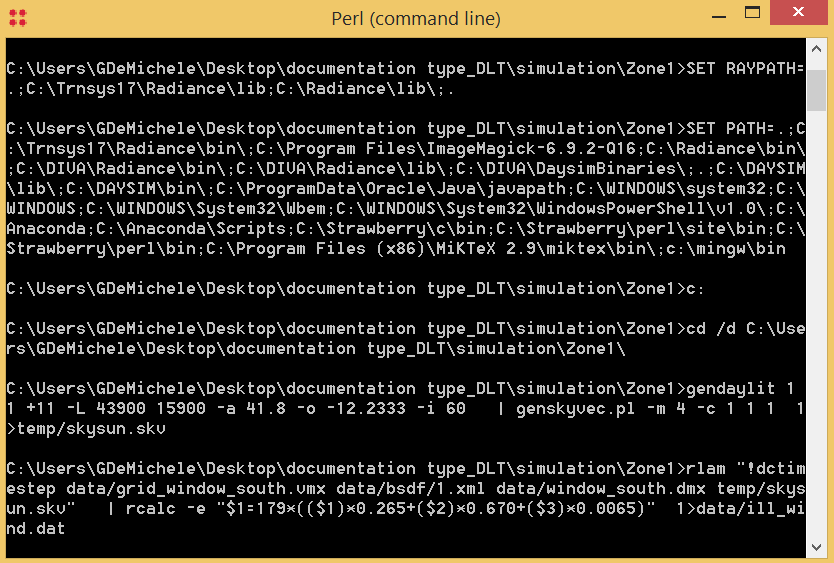
\includegraphics[width=0.9\textwidth]{3pm}
\caption{\label{img1:3pm} Three-Phase method description}
\end{figure}



The equations that describe the process are:

\begin{equation}\label{eq1:hour}
i= VTD s 
\end{equation}

\begin{equation}
 I = VTD S
\end{equation}

where, by \cite{3ph_tut} :
\begin{itemize}
\item i = point in time illuminance or luminance result;
\item I = matrix containing time series of illuminance or luminance result, annual simulation;
\item V= view matrix, relating outgoing directions on window to desired results at interior;
\item T = transmission matrix, relating incident window directions to exiting directions (BSDF);
\item D = daylight matrix, relating sky patches to incident directions on window;
\item s = sky vector, assigning luminance values to patches representing sky directions;
\item S = sky matrix, a collection of sky vectors.
\end{itemize}

The V and D matrices are created with a Radiance simulation. The T matrix can be created using LBNL 
WINDOW software, by simulation (e.g. TracePro or Radiance genBSDF) or can be measured with a 
goniophotometer. The s vector and S matrix are generated from a Radiance sky description \cite{3ph_tut}.
Once evaluate the V,D and T matrix, that require a quite long time, these do not must be again calculated. Then the matrix multiplication is very fast, and in few second gives the results.\\

In particular, TypeDLT uses the equation \ref{eq1:hour} hourly-based. This strategy increases the calculation time but allows to connect the results of the daylighting simulation after each time step with the other Types onto the TRNSYS deck.





%Radiance is validated software for the lighting and daylighting modelling able to perform daylighting simulations climate-based using the BSDF data that characterize the shading device. This is possible thanks to a very fast calculation method, called Three-Phase Method, in which the passage of the ray light from the sky dome to the sensors is divided in three steps (Figure \ref{img1:3pm}).
%The algorithm is based on the matrix equation

